\documentclass[../Thesis-IJspeert.tex]{subfiles}

\begin{document}

\graphicspath{ {"Strong Coupling in an Atom-Cavity System/figs/"} }
\pgfplotsset{table/search path={"Strong Coupling in an Atom-Cavity System/data/"}}

\chapter{Strong Coupling in an Atom-Cavity System}
\addtocontents{toc}{\vskip-6pt\par\noindent\protect\textcolor{gray75}{\protect\rule{\textwidth}{0.5pt}}\par}
\label{chap:StrongCouplinginanAtom-CavitySystem}

\section{Entanglement of single atoms using optical cavities}
A standard approach for entangling two distant atoms relies on the interference of narrow-band indistinguishable photons, emitted from two atom-cavity systems. \autoref{fig:entangle} illustrates a particular entangling scheme in which two single \ce{^87Rb} atoms are coupled to optical cavities and prepared in the $\ket{F=2,m_F=0}$ state of the \ce{5\!^2S_{\sfrac{1}{2}}} ground level.
\begin{figure}[h]
	\centering
	\begin{tikzpicture}
	\node[anchor=south west,inner sep=0] (image) at (0,0) {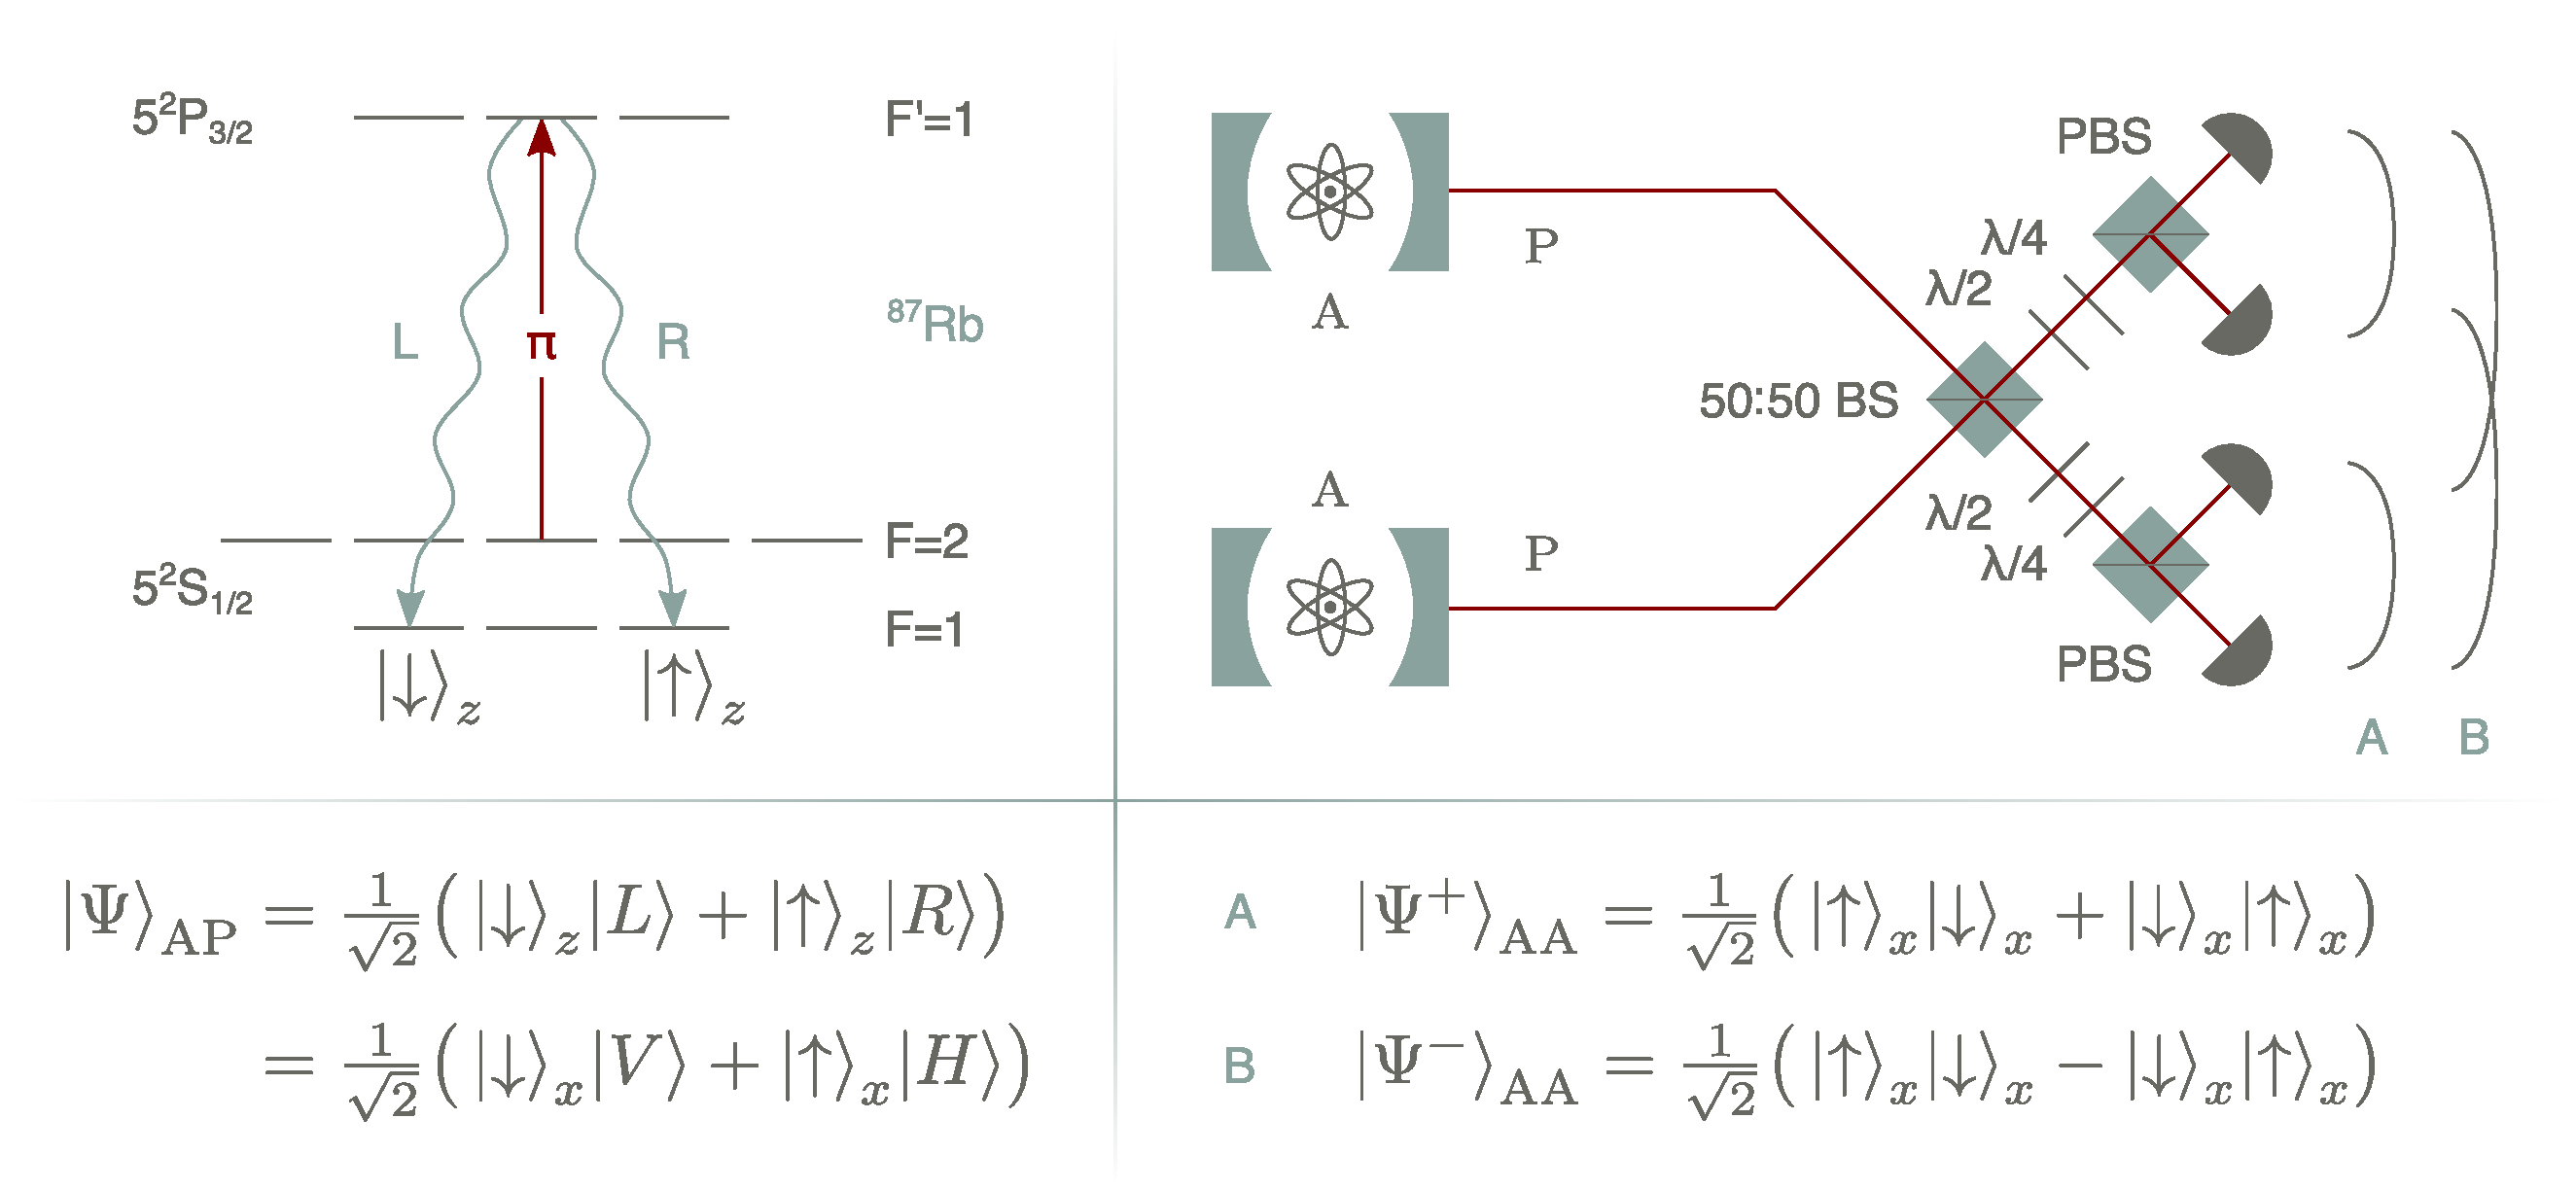
\includegraphics[width=1\textwidth]{entangle2.pdf}};
	\begin{scope}[x={(image.south east)},y={(image.north west)}]
	
	%\draw[help lines,xstep=.1,ystep=.1] (0,0) grid (1,1);
	%\foreach \x in {0,1,...,9} { \node [anchor=north] at (\x/10,0) {0.\x}; }
	%\foreach \y in {0,1,...,9} { \node [anchor=east] at (0,\y/10) {0.\y}; }
	
	\node[rectangle, rounded corners=1mm, minimum size=5mm, text width=55mm,
	anchor=base, very thick, draw=none, fill=white, align=left] at (0.20,0.215) {\small\textcolor{markgrijs}{$ \color{markgrijs} \ket{\Psi}_\text{AP} = \frac{1}{\sqrt{2}} \big( \ket{\downarrow}_z\!\ket{\sigma^+} + \ket{\uparrow}_z\!\ket{\sigma^-} \! \big) $}};
	
	\node[rectangle, rounded corners=1mm, minimum size=5mm, text width=55mm,
	anchor=base, very thick, draw=none, fill=white, align=left] at (0.20,0.0850) {\small\textcolor{markgrijs}{$ \color{white} \ket{\Psi}_\text{AP} \color{markgrijs}= \frac{1}{\sqrt{2}} \big( \ket{\downarrow}_x\!\ket{V} + \ket{\uparrow}_x\!\ket{H} \! \big)$}};
	
	\node[rectangle, rounded corners=1mm, minimum size=5mm, text width=5mm,
	anchor=base, very thick, draw=none, fill=white, align=left] at (0.168,0.395) {\small\textcolor{markgrijs}{$ \ket{\downarrow}_z\!$}};	
	
	\node[rectangle, rounded corners=1mm, minimum size=5mm, text width=5mm,
	anchor=base, very thick, draw=none, fill=white, align=left] at (0.272,0.395) {\small\textcolor{markgrijs}{$ \ket{\uparrow}_z\!$}};		
	
	\node[rectangle, rounded corners=1mm, minimum size=5mm, text width=3mm,
	anchor=base, very thick, draw=none, fill=white, align=left] at (0.15,0.7) {\small\textcolor{markviesblauw}{$ \sigma^+$}};	
	
	\node[rectangle, rounded corners=1mm, minimum size=5mm, text width=3mm,
	anchor=base, very thick, draw=none, fill=white, align=left] at (0.265,0.7) {\small\textcolor{markviesblauw}{$ \sigma^-$}};	
	
	\node[rectangle, rounded corners=1mm, minimum size=5mm, text width=2mm,
	anchor=base, very thick, draw=none, fill=white, align=left] at (0.21,0.7) {\small\textcolor{markrood}{$ \pi$}};	
	
	\node[rectangle, rounded corners=1mm, minimum size=5mm, text width=60mm,
	anchor=base, very thick, draw=none, fill=white, align=left] at (0.74,0.215) {\small\textcolor{markgrijs}{$ \color{markgrijs} \ket{\Psi^+}_\text{AA} = \frac{1}{\sqrt{2}} \big( \ket{\uparrow}_x\!\ket{\downarrow}_x + \ket{\downarrow}_x\!\ket{\uparrow}_x \! \big) $}};
	
	\node[rectangle, rounded corners=1mm, minimum size=5mm, text width=60mm,
	anchor=base, very thick, draw=none, fill=white, align=left] at (0.74,0.085) {\small\textcolor{markgrijs}{$ \color{markgrijs} \ket{\Psi^-}_\text{AA} = \frac{1}{\sqrt{2}} \big( \ket{\uparrow}_x\!\ket{\downarrow}_x - \ket{\downarrow}_x\!\ket{\uparrow}_x \! \big) $}};
	
	%\node[rectangle, rounded corners=1mm, minimum size=5mm, text width=2mm,
	%anchor=base, very thick, draw=markviesblauw, fill=markviesblauw, align=center] at (0.4,0.385) {\small\textcolor{white}{\textbf{a}}};
	
	%\node[rectangle, rounded corners=1mm, minimum size=5mm, text width=2mm,
	%anchor=base, very thick, draw=markviesblauw, fill=markviesblauw, align=center] at (0.4,0.235) {\small\textcolor{white}{\textbf{b}}};
	
	%\node[rectangle, rounded corners=1mm, minimum size=5mm, text width=2mm,
	%anchor=base, very thick, draw=markviesblauw, fill=markviesblauw, align=center] at (0.465,0.385) {\small\textcolor{white}{\textbf{c}}};
	
	%\node[rectangle, rounded corners=1mm, minimum size=5mm, text width=2mm,
	%anchor=base, very thick, draw=markviesblauw, fill=markviesblauw, align=center] at (0.465,0.235) {\small\textcolor{white}{\textbf{d}}};
	
	\end{scope}
	\end{tikzpicture}
	\caption[An example of a floating figure]{Entangling scheme for two \ce{^87Rb} atoms. Each atom undergoes vacuum-stimulated Raman adiabatic passage (top left), which results in an atom-photon entangled state (bottom left). A bell state measurement of the emitted photon pair (top right) projects the atoms onto a maximally entangled state (bottom right).} % The text in the square bracket is the caption for the list of figures while the text in the curly brackets is the figure caption
	\label{fig:entangle} 
\end{figure}
The cavity axis is chosen as the quantisation direction (\autoref{fig:cavity}).
\begin{figure}[t]
	\centering
	\begin{tikzpicture}
	\node[anchor=south west,inner sep=0] (image) at (0,0) {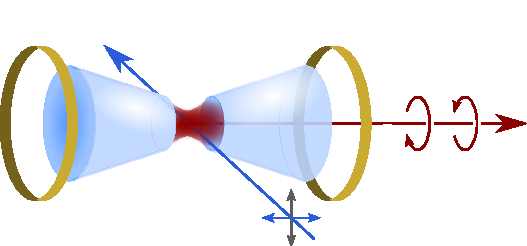
\includegraphics[width=0.5\textwidth]{cavity2.pdf}};
	\begin{scope}[x={(image.south east)},y={(image.north west)}]
	
	%\draw[help lines,xstep=.1,ystep=.1] (0,0) grid (1,1);
	%\foreach \x in {0,1,...,9} { \node [anchor=north] at (\x/10,0) {0.\x}; }
	%\foreach \y in {0,1,...,9} { \node [anchor=east] at (0,\y/10) {0.\y}; }
	%\node[] at (0.16,1.05) {\small\textcolor{markgoud}{$B$}};
	\node[] at (0.33,0.03) {\small\textcolor{markgrijs}{$V\rightarrow \sigma^++\sigma^-$}};
	\node[] at (0.33,0.18) {\small\textcolor{markdiepblauw}{$H\rightarrow \pi$}};
	\node[] at (0.8,0.28) {\small\textcolor{markrood}{$\sigma^+$}};
	\node[] at (0.89,0.28) {\small\textcolor{markrood}{$\sigma^-$}};
	\end{scope}
	\end{tikzpicture}
	\caption[An example of a floating figure]{The quantisation direction (yellow) along the axis of an optical cavity, which only supports the $\sigma^+$ and $\sigma^-$ polarisation modes (red). A perpendicular laser (blue) drives $\pi$ and $\sigma^+/\sigma^-$ transitions for horizontally and vertically polarised light respectively. The two anti-Helmholtz coils are necessary for generating a magneto-optical trap (not shown).} % The text in the square bracket is the caption for the list of figures while the text in the curly brackets is the figure caption
	\label{fig:cavity} 
\end{figure}
The cavity, which supports the right circular ($\sigma^+$ ) and left circular ($\sigma^-$) polarisation modes, couples $\ket{F=1}$ and $\ket{F'=1}$ of the \ce{5\!^2P_{\sfrac{3}{2}}} excited level. Together with a $\pi$-polarised laser resonant with the $\ket{F=2}\leftrightarrow \ket{F'=1}$ transition, this allows for a vacuum-stimulated Raman adiabatic passage to $\ket{\downarrow}_z:=\ket{F=1,m_F=-1}$ or $\ket{\uparrow}_z:=\ket{F=1,m_F=1}$ in the ground state. This results in the generation of a $\sigma^+$ or $\sigma^-$ photon and leaves both atom-photon systems in the following entangled state:
\begin{equation}
\color{black} \ket{\Psi}_\text{AP} = \frac{1}{\sqrt{2}} \big( \ket{\downarrow}_z\!\ket{\sigma^+} + \ket{\uparrow}_z\!\ket{\sigma^-} \! \big) \,.
\end{equation}
A subsequent Bell state measurement of the two photons from both systems is based on the Hong-Ou-Mandel effect \cite{HOM} and projects the atoms onto one of two distinguishable, maximally entangled states:
\begin{equation}
\begin{split}
\color{black} \ket{\Psi^+}_\text{AA} = \frac{1}{\sqrt{2}} \big( \ket{\uparrow}_x\!\ket{\downarrow}_x + \ket{\downarrow}_x\!\ket{\uparrow}_x \! \big) \,, \\ \color{black} \ket{\Psi^-}_\text{AA} = \frac{1}{\sqrt{2}} \big( \ket{\uparrow}_x\!\ket{\downarrow}_x - \ket{\downarrow}_x\!\ket{\uparrow}_x \! \big) \,.
\end{split}
\end{equation}
This constitutes a probabilistic\footnote{Alternatively, a deterministic entangling scheme is based on the absorption of an emitted photon by the second atom, see \cite{Dilley2012}.} procedure, as it requires a projective measurement of the emitted photon pair. This procedure of entangling two trapped \ce{^87Rb} atoms has been successfully tested without the use of optical cavities \cite{Hofmann2012}. However, the atom-photon coupling can be strengthened significantly by placing the emitter in a high-finesse optical cavity \cite{Specht2011,Hijlkema2007}. This supports deterministic photon emission into a single mode of the radiation field through what is known as the Purcell effect \cite{Purcell1946}. The potential of a cavity-enhanced atom-photon interface for the delivery of single photons and distributed entanglement has been demonstrated using \ce{^87Rb} atoms stochastically loaded into a high-finesse optical cavity \cite{Barrett2019}. However, the nature of atomic loading in this experiment gives rise to time-dependent coupling strengths and limits the overall production efficiency of photons. In addition, stochastic loading becomes ineffective when multiple cavities must be filled simultaneously (see \autoref{appendixA}).

	
\end{document}